\section{Vorhandene Partitionen formatieren und zur Installation nutzen}
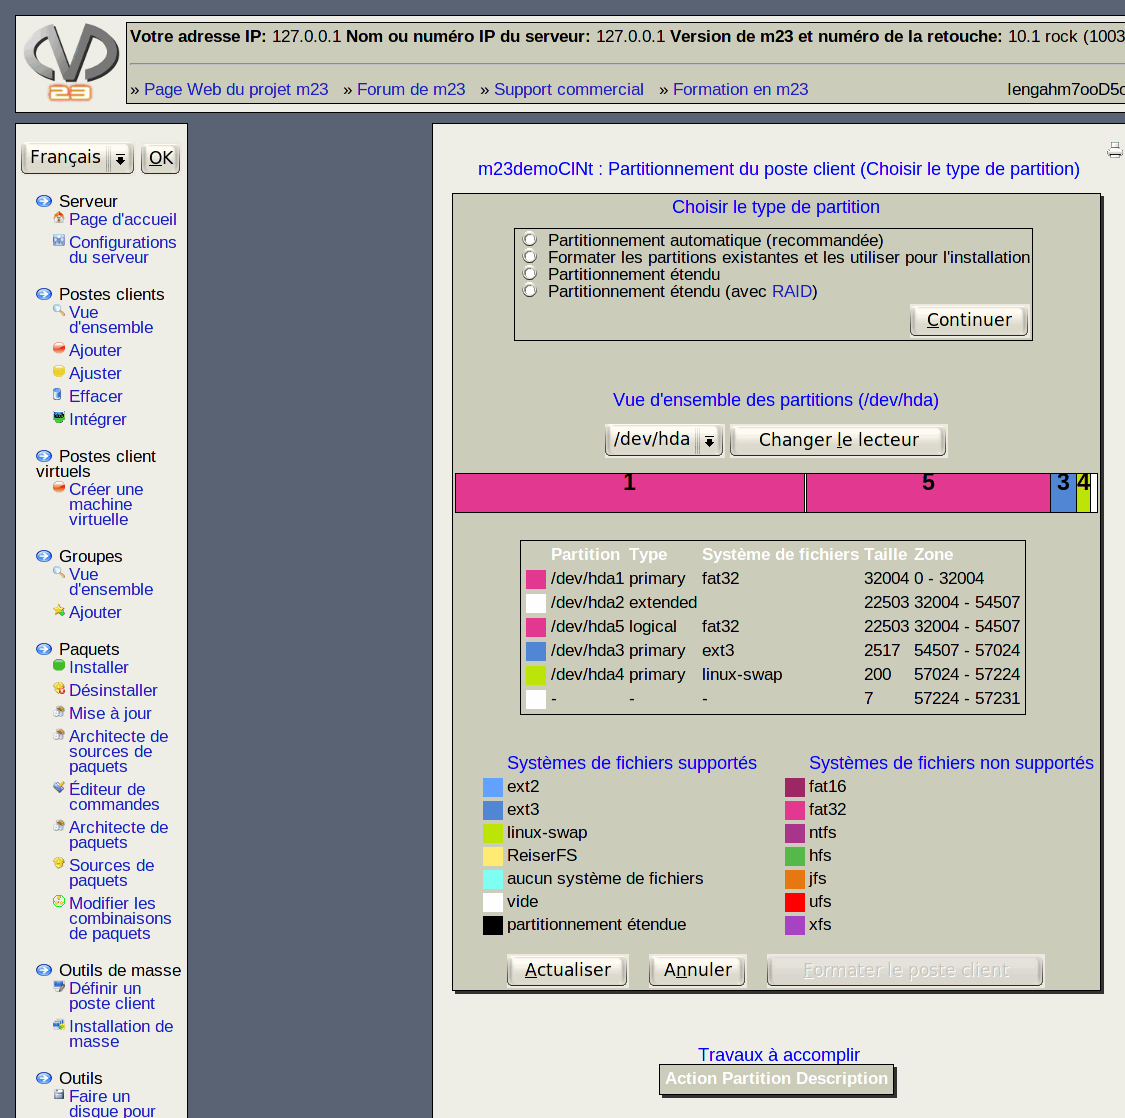
\includegraphics[scale=0.4]{/mdk/doc/manual/screenshots/de/fdisk-existing.png} \\
Diese Option bietet Ihnen die M�glichkeit, vorhandene Partitionen neu zu formatieren und f�r die Installation zu nutzen. Sie w�hlen zwei Partitionen aus. Die erste, um das Betriebssystem zu installieren und die zweite als Auslagerungsplatz (Swap).\\
\subsection{Schrittweises Vorgehen:}
\begin{enumerate}
\item W�hlen Sie \textit{"Vorhandene Partitionen formatieren und zur Installation nutzen"}
\item W�hlen Sie dann die Partitionen, die Sie zur Installation und zum Swappen nutzen m�chten.\\
\item Durch Klicken des \textit{"Aktualisieren"}-Buttons k�nnen Sie die Partitionierung begutachten\\
\item Klicken Sie auf \textit{"Client formatieren"}, um die Angaben zu �bernehmen\\
\end{enumerate}
